\section{Introduction}
\label{sec:section}
  Keyphrases are single or multi-word expressions that represent the main topics
  of a document. Keyphrases are useful in many tasks such as information
  retrieval~\cite{medelyan2008smalltrainingset}, document
  summarization~\cite{litvak2008graphbased} or document
  clustering~\cite{han2007webdocumentclustering}. Although scientific articles
  usually provide them, most of the documents have no associated keyphrases.
  Therefore, the problem of automatically assigning keyphrases to documents is
  an active field of research.

  Automatic keyphrase extraction methods are divided into two categories:
  supervised and unsupervised methods. Supervised methods typically recast
  keyphrase extraction as a binary classification
  task~\cite{witten1999kea,sujian2003maximumentropy,eichler2010keywe}. For
  unsupervised methods, keyphrase extraction is often considered as a ranking
  task and many approaches are
  used~\cite{barker2000nounphrasehead,tomokiyo2003languagemodel,mihalcea2004textrank}.
  As distinct as they are, both supervised and unsupervised methods rely on a
  preliminary candidate extraction step which identifies single and multi-word
  expressions that have the same syntactic properties than a keyphrase. These
  expressions are the only textual units that can be extracted as keyphrases.
  
  In this paper, we focus on the candidate extraction step and show its impact
  on the performance of automatic keyphrase extraction. Various methods
  are commonly employed to extract keyphrase candidates\footnote{In this work,
  we do not consider methods which use a manually defined controlled
  vocabulary.}. Usually, a set of either single words, n-grams filtered by stop
  words, NP-chunks or sequences of words matching given patterns is
  extracted~\cite{hulth2003keywordextraction}. According to the chosen method,
  the extracted set contains more or less candidates, and the amount of these
  that match with the ground truth keyphrases may vary. Hence, a few questions
  arise. How the different sets influence the keyphrase extraction? Do large
  candidate sets introduce noise that affects the performance of some keyphrase
  extraction methods?

  We seek to better understand the impact of candidate extraction methods on
  keyphrase extraction by studying the aforementioned questions. We first
  quantify the differences between the candidate sets obtained by the commonly
  used methods. Also, we propose to use another method developed to extract
  noun-phrases for document indexing~\cite{evans1996nounphraseanalysis} and we
  argue that such term detection
  method~\cite{castellvi2001automatictermdetection} provides solid keyphrase
  candidates. Then, we evaluate the impact of the candidate extraction methods
  on three dissimilar keyphrase extraction methods. We select
  KEA~\cite{witten1999kea} to represent supervised methods,
  TF-IDF~\cite{jones1972tfidf} to represent unsupervised methods that require a
  collection of documents and TopicRank~\cite{bougouin2013topicrank} to
  represent unsupervised methods that only make use of the document to analyse.

  \todo[inline]{Results show that...}

\section{Definition of Candidate Keyphrases}
\label{sec:study_of_ground_truth_keyphrases}
  Candidate keyphrases are textual units which can be selected as keyphrases
  of the document they are extracted from. Hence, they must have the same
  syntactic and linguistic properties than ground truth keyphrases. This section
  aims to determine those properties by analysing three standard evaluation
  datasets, for keyphrase extraction, and by providing statistics about their
  reference keyphrases (ground truth keyphrases).

  \subsection{Keyphrase Extraction Datasets}
  \label{subsec:keyphrase_extraction_datasets}
    Keyphrase extraction datasets are used to train or evaluate keyphrase
    extraction methods. Hence, the datasets are collections of documents paired
    with reference keyphrases, given by authors, readers or both. Unlike the
    studied methods, human annotators do not only extract keyphrases which are
    contained into the document. This problem of missing keyphrases leads to a
    bias of the training or evaluation of keyphrase extraction methods. In this
    work, we use three standard datasets which differ in terms of document type
    and/or language. The problem of missing keyphrases is partially bypassed
    using their stemmed forms during comparisons, when training or evaluating
    methods.

    The \textbf{DUC} dataset \cite{over2001duc} is a collection of 308 English
    news articles covering about 30 news topics. This is the part of the dataset
    made for the DUC 2001 summarization evaluation campaign that has been
    annotated by \newcite{wan2008expandrank} for keyphrase extraction evaluation
    purpose. We split this into two sets: a training set containing 208
    documents and a test set containing 100 documents.

    The \textbf{SemEval} dataset \cite{kim2010semeval} contains 284 English
    papers collected from the ACM Digital Libraries (conference and workshop
    papers). The 284 scientific papers are divided into three sets: a trial set
    containing 40 documents (unused in this work), a training set containing 144
    documents and a test set containing 100 documents. As for the associated
    keyphrases, these are provided by both authors and readers.

    The \textbf{DEFT} dataset \cite{Paroubek2012deft} is a collection of 244
    French scientific papers that belongs to the Humanities and Social Sciences
    domain. As SemEval, DEFT is divided into threee sets: a trial set containing
    50 documents (not used in this work), a training set containing 141
    documents and a test set containing 93 documents. Unlike DUC and SemEval,
    the only available reference keyphrases are the ones given by authors.

    Table \ref{tab:dataset_statistics} gives statistics about the datasets. As
    we aim to use these statistics to lead this work, we restrain the discussion
    to observations made with the training sets.\todo{Continue}
    \begin{table*}
      \centering
      \begin{tabular}{rrccc}
        \toprule
        & \multirow{2}{*}[-2pt]{\textbf{Statistics}} & \multicolumn{3}{c}{\textbf{Corpora}}\\
        \cmidrule{3-5}
        & & DUC & SemEval & DEFT\\
        \midrule
        \multirow{6}{*}[-2pt]{\begin{sideways}\textbf{Documents}\end{sideways}} & Language & English & English & French\\
        & Type & News & Papers & Papers\\
        & Documents & 208 & 144 & 141\\
        & Tokens/document & & 5134.6 & 7276.7\\
        & Keyphrases/document & 8.1 & 15.4 & 5.4\\
        & Missings keyphrases & & 13.5\% & 18.2\%\\
        \addlinespace[\defaultaddspace]
        \multirow{11}{*}[-2pt]{\begin{sideways}\textbf{Keyphrases}\end{sideways}} & Unigrams & 26.2\% & 20.2\% & 66.4\%\\
        & Bigrams & 54.1\% & 53.4\% & 20.7\%\\
        & Trigrams and more & 19.7\% & 26.4\% & 12.9\%\\
        & Containing nouns & 90.8\% & 95.9\% & 79.3\%\\
        & Containing proper nouns & 18.7\% & $~~$5.8\% & 16.8\%\\
        & Containing adjectives & 41.6\% & 40.5\% & 28.8\%\\
        & Containing verbs & $~~$0.9\% & $~~$3.4\% & $~~$0.5\%\\
        & Containing adverbs & $~~$1.3\% & $~~$0.6\% & $~~$0.5\%\\
        & Containing prepositions & $~~$0.2\% & $~~$1.2\% & 12.7\%\\
        & Containing determiners & $~~$0.0\% & $~~$0.0\% & $~~$8.1\%\\
        & Containing others & $~~$1.3\% & $~~$2.1\% & $~~$5.8\%\\
        \bottomrule
      \end{tabular}
      \caption{Training dataset statistics. As a matter of consistency regarding
               the training and the evaluation of keyphrase extraction methods,
               the percentage of missing keyphrase is determined based on the
               stemmed form of the reference keyphrases.
               \label{tab:dataset_statistics}}
    \end{table*}

  \subsection{Keyphrase Analysis}
  \label{subsec:keyphrase_analysis}
    This section focuses on the reference keyphrase statistics presented in
    Table \ref{tab:dataset_statistics}. The aim is to determine the syntactic
    properties of most keyphrases, for English (combining information from DUC
    and SemEval) and for French (using DEFT information).

    \todo[inline]{- Les Keyphrases sont principalement des uni-grammes et
                  bi-grammes (mais une tendance inversée entre anglais et
                  français). - Presque toutes les keyphrase contiennent un nom.
                  - L'usage d'adjectifs est fréquent (40 et 30\%). - Très peu de
                  verbes. - Usage fréquent de prépositions et determinants pour
                  le français (uniquement).\\\begin{center}DONNER DES
                  EXEMPLES\end{center}}
    \todo[inline]{Donner les séquences de POS les plus fréquentes dans le gold
                  standard.}

\section{Candidate Extraction}
\label{sec:candidate_extraction}
  \todo[inline]{Objectif + pré-requis.}

  \subsection{N-Gram Extraction}
  \label{subsec:n_gram_extraction}
  \subsection{NP-Chunk Extraction}
  \label{subsec:np_chunk_extraction}
  \subsection{Pattern Matching}
  \label{subsec:pattern_matching}
  \subsection{Term Extraction}
  \label{subsec:term_extraction}

\section{Keyphrase Extraction}
\label{sec:keyphrase_extraction}
  \todo[inline]{Fonctionnement général.}
  \begin{figure}
    \centering
    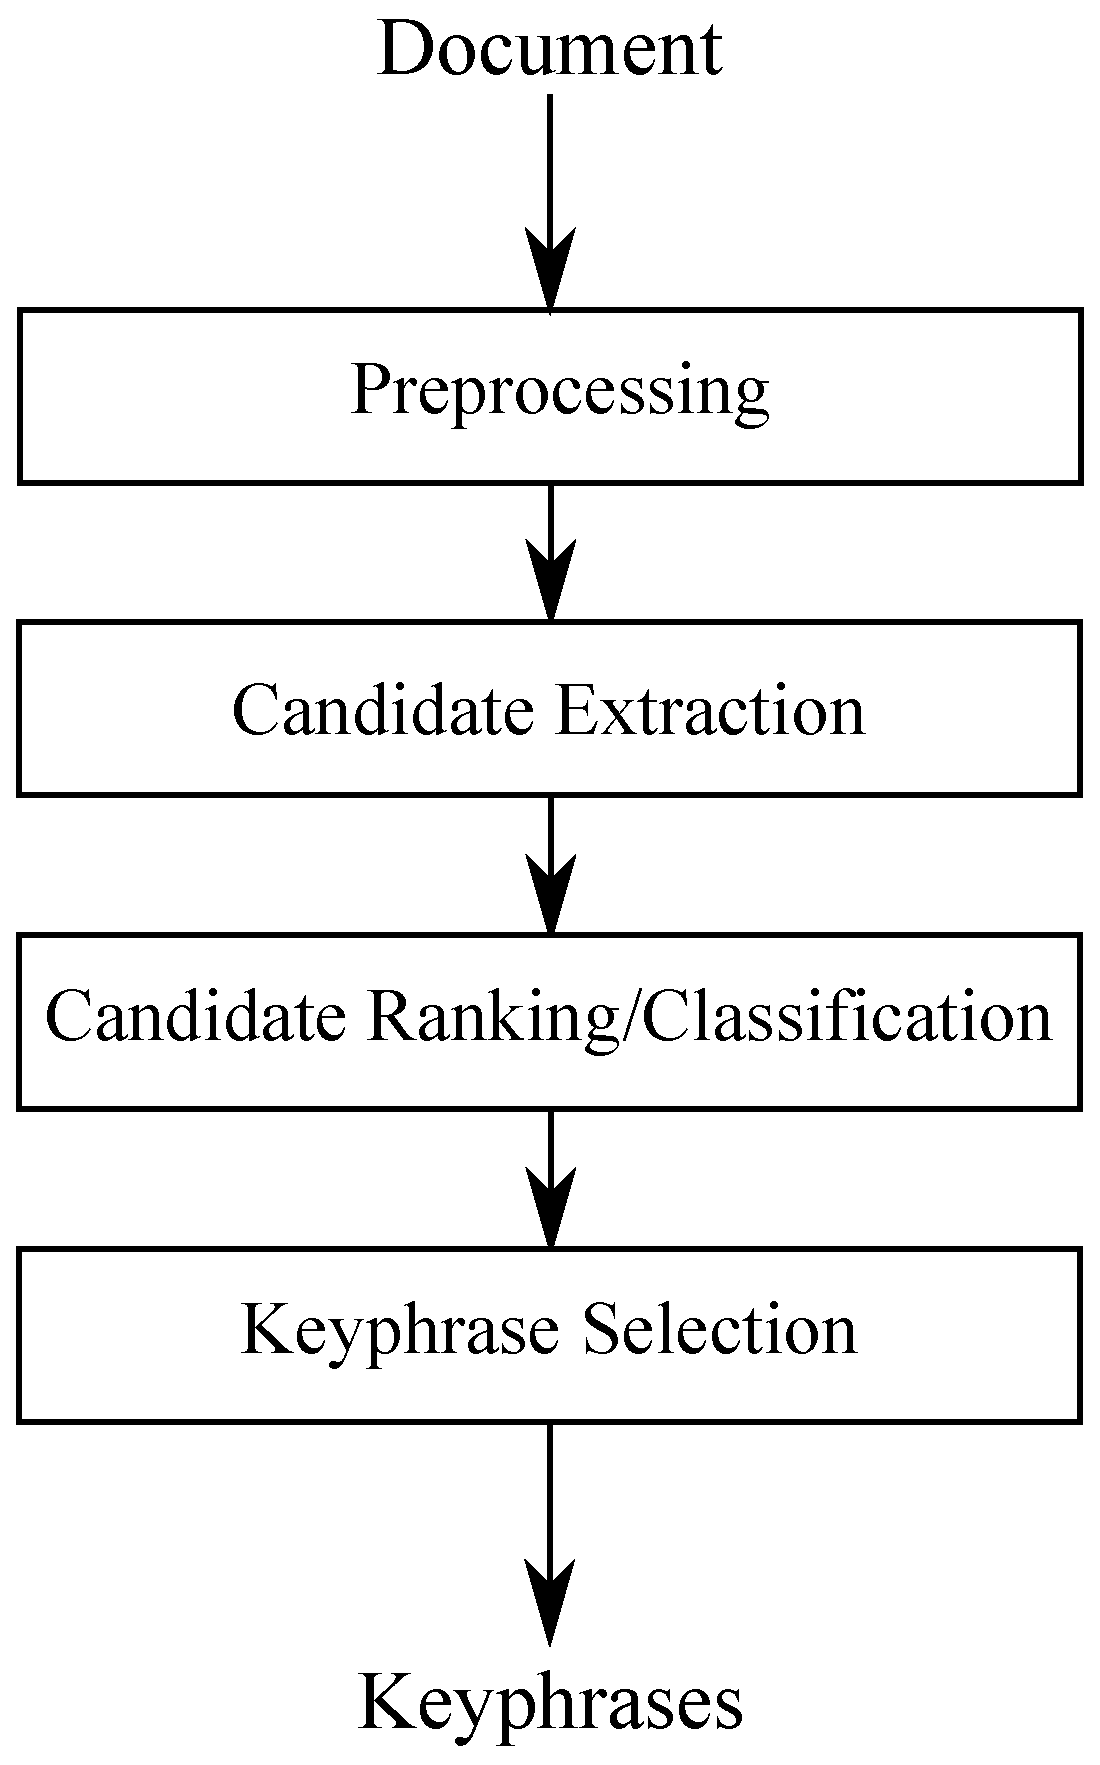
\includegraphics[width=0.3\textwidth]{include/processing_steps.eps}
    \caption{Processing steps of automatic keyphrase extraction methods.
             \label{fig:processing_steps}}
  \end{figure}

  \subsection{TF-IDF}
  \label{subsec:tfidf}
  \subsection{TopicRank}
  \label{subsec:topicrank}
  \subsection{KEA}
  \label{subsec:kea}

\section{Evaluation}
\label{sec:evaluation}
  \todo[inline]{Expliquer les deux évaluations: intrinsèque et extrinsèque.}

  \subsection{Experimental Setting}
  \label{subsec:experimental_setting}
    \begin{table*}
      \centering
      \begin{tabular}{rccc}
        \toprule
        \multirow{2}{*}[-2pt]{\textbf{Statistics}} & \multicolumn{3}{c}{\textbf{Corpora}}\\
        \cmidrule{2-4}
        & DUC & SemEval & DEFT\\
        \midrule
        Language & English & English & French\\
        Type & News & Papers & Papers\\
        Documents & 100 & 100 & 93\\
        Tokens/document & & 5179.6 & 6844.0\\
        Keyphrases/document & & 14.7 & 5.2\\
        Missings keyphrases & & & \\
        \bottomrule
      \end{tabular}
      \caption{Test dataset statistics. As a matter of consistency regarding
               the training and the evaluation of keyphrase extraction methods,
               the percentage of missing keyphrase is determined based on the
               stemmed form of the reference keyphrases.
               \label{tab:dataset_statistics}}
    \end{table*}

  \subsection{Candidate Extraction}
  \label{subsec:candidate_extraction}
    \todo[inline]{Donner le rappel max et comparer avec la taille des différents
                  ensemble.}

    \begin{table*}[h]
      \centering
      \begin{tabular}{rcccccc}
        \toprule
        \multirow{2}{*}[-2pt]{\textbf{Methods}} & \multicolumn{2}{c}{\textbf{DUC}} & \multicolumn{2}{c}{\textbf{SemEval}} & \multicolumn{2}{c}{\textbf{DEFT}}\\
        \cmidrule(r){2-3}\cmidrule(lr){4-5}\cmidrule(l){6-7}
        & Candidates & Rmax & Candidates & Rmax & Candidates & Rmax\\
        \midrule
        \{1..2\}-grams\\
        \{1..3\}-grams\\
        \{1..4\}-grams\\
        \{1..5\}-grams\\
        NP chunks\\
        Longest NPs\\
        Best patterns\\
        TermSuite\\
        CLARIT'96\\
        \bottomrule
      \end{tabular}
      \caption{Candidate extraction statistics. Rmax stands for maximum recall,
               i.e. it is the percentage of candidates that match with reference
               keyphrases. \label{tab:candidate_extraction_statistics}}
    \end{table*}

    \todo[inline]{Quels sont les termes candidats communs aux ensembles, les
                  propriétés ?}

  \subsection{Keyphrase Extraction}
  \label{subsec:keyphrase_extraction}
    \todo[inline]{Quelles sont les performances de chaque méthode avec chaque
                  ensemble de termes candidats ?}

    \begin{table*}[h]
      \centering
      \begin{tabular}{rccccccccc}
        \toprule
        \multirow{2}{*}[-2pt]{\textbf{Methods}} & \multicolumn{3}{c}{\textbf{DUC}} & \multicolumn{3}{c}{\textbf{SemEval}} & \multicolumn{3}{c}{\textbf{DEFT}}\\
        \cmidrule(r){2-4}\cmidrule(lr){5-7}\cmidrule(l){8-10}
        & P & R & F & P & R & F & P & R & F\\
        \midrule
        \{1..2\}-grams & ${~~}$00.0 & ${~~}$00.0 & ${~~}$00.0 & ${~~}$00.0 & ${~~}$00.0 & ${~~}$00.0 & ${~~}$00.0 & ${~~}$00.0 & ${~~}$00.0\\
        \{1..3\}-grams & ${~~}$00.0 & ${~~}$00.0 & ${~~}$00.0 & ${~~}$00.0 & ${~~}$00.0 & ${~~}$00.0 & ${~~}$00.0 & ${~~}$00.0 & ${~~}$00.0\\
        \{1..4\}-grams & ${~~}$00.0 & ${~~}$00.0 & ${~~}$00.0 & ${~~}$00.0 & ${~~}$00.0 & ${~~}$00.0 & ${~~}$00.0 & ${~~}$00.0 & ${~~}$00.0\\
        \{1..5\}-grams & ${~~}$00.0 & ${~~}$00.0 & ${~~}$00.0 & ${~~}$00.0 & ${~~}$00.0 & ${~~}$00.0 & ${~~}$00.0 & ${~~}$00.0 & ${~~}$00.0\\
        NP chunks & ${~~}$00.0 & ${~~}$00.0 & ${~~}$00.0 & ${~~}$00.0 & ${~~}$00.0 & ${~~}$00.0 & ${~~}$00.0 & ${~~}$00.0 & ${~~}$00.0\\
        Longest NPs & ${~~}$00.0 & ${~~}$00.0 & ${~~}$00.0 & ${~~}$00.0 & ${~~}$00.0 & ${~~}$00.0 & ${~~}$00.0 & ${~~}$00.0 & ${~~}$00.0\\
        Best patterns & ${~~}$00.0 & ${~~}$00.0 & ${~~}$00.0 & ${~~}$00.0 & ${~~}$00.0 & ${~~}$00.0 & ${~~}$00.0 & ${~~}$00.0 & ${~~}$00.0\\
        TermSuite & ${~~}$00.0 & ${~~}$00.0 & ${~~}$00.0 & ${~~}$00.0 & ${~~}$00.0 & ${~~}$00.0 & ${~~}$00.0 & ${~~}$00.0 & ${~~}$00.0\\
        CLARIT'96 & ${~~}$00.0 & ${~~}$00.0 & ${~~}$00.0 & ${~~}$00.0 & ${~~}$00.0 & ${~~}$00.0 & ${~~}$00.0 & ${~~}$00.0 & ${~~}$00.0\\
        \bottomrule
      \end{tabular}
      \caption{Comparison of candidate extraction methods, when extracting 10
               keyphrases with the \textbf{TF-IDF} method. Results are expressed
               as a percentage of precision (P), recall (R) and f-score (F).
               \label{tab:keyphrase_extraction_results}}
    \end{table*}

    \begin{table*}[h]
      \centering
      \begin{tabular}{rccccccccc}
        \toprule
        \multirow{2}{*}[-2pt]{\textbf{Methods}} & \multicolumn{3}{c}{\textbf{DUC}} & \multicolumn{3}{c}{\textbf{SemEval}} & \multicolumn{3}{c}{\textbf{DEFT}}\\
        \cmidrule(r){2-4}\cmidrule(lr){5-7}\cmidrule(l){8-10}
        & P & R & F & P & R & F & P & R & F\\
        \midrule
        \{1..2\}-grams & ${~~}$00.0 & ${~~}$00.0 & ${~~}$00.0 & ${~~}$00.0 & ${~~}$00.0 & ${~~}$00.0 & ${~~}$00.0 & ${~~}$00.0 & ${~~}$00.0\\
        \{1..3\}-grams & ${~~}$00.0 & ${~~}$00.0 & ${~~}$00.0 & ${~~}$00.0 & ${~~}$00.0 & ${~~}$00.0 & ${~~}$00.0 & ${~~}$00.0 & ${~~}$00.0\\
        \{1..4\}-grams & ${~~}$00.0 & ${~~}$00.0 & ${~~}$00.0 & ${~~}$00.0 & ${~~}$00.0 & ${~~}$00.0 & ${~~}$00.0 & ${~~}$00.0 & ${~~}$00.0\\
        \{1..5\}-grams & ${~~}$00.0 & ${~~}$00.0 & ${~~}$00.0 & ${~~}$00.0 & ${~~}$00.0 & ${~~}$00.0 & ${~~}$00.0 & ${~~}$00.0 & ${~~}$00.0\\
        NP chunks & ${~~}$00.0 & ${~~}$00.0 & ${~~}$00.0 & ${~~}$00.0 & ${~~}$00.0 & ${~~}$00.0 & ${~~}$00.0 & ${~~}$00.0 & ${~~}$00.0\\
        Longest NPs & ${~~}$00.0 & ${~~}$00.0 & ${~~}$00.0 & ${~~}$00.0 & ${~~}$00.0 & ${~~}$00.0 & ${~~}$00.0 & ${~~}$00.0 & ${~~}$00.0\\
        Best patterns & ${~~}$00.0 & ${~~}$00.0 & ${~~}$00.0 & ${~~}$00.0 & ${~~}$00.0 & ${~~}$00.0 & ${~~}$00.0 & ${~~}$00.0 & ${~~}$00.0\\
        TermSuite & ${~~}$00.0 & ${~~}$00.0 & ${~~}$00.0 & ${~~}$00.0 & ${~~}$00.0 & ${~~}$00.0 & ${~~}$00.0 & ${~~}$00.0 & ${~~}$00.0\\
        CLARIT'96 & ${~~}$00.0 & ${~~}$00.0 & ${~~}$00.0 & ${~~}$00.0 & ${~~}$00.0 & ${~~}$00.0 & ${~~}$00.0 & ${~~}$00.0 & ${~~}$00.0\\
        \bottomrule
      \end{tabular}
      \caption{Comparison of candidate extraction methods, when extracting 10
               keyphrases with \textbf{TopicRank}. Results are expressed as a
               percentage of precision (P), recall (R) and f-score (F).
               \label{tab:keyphrase_extraction_results}}
    \end{table*}

    \begin{table*}[h]
      \centering
      \begin{tabular}{rccccccccc}
        \toprule
        \multirow{2}{*}[-2pt]{\textbf{Methods}} & \multicolumn{3}{c}{\textbf{DUC}} & \multicolumn{3}{c}{\textbf{SemEval}} & \multicolumn{3}{c}{\textbf{DEFT}}\\
        \cmidrule(r){2-4}\cmidrule(lr){5-7}\cmidrule(l){8-10}
        & P & R & F & P & R & F & P & R & F\\
        \midrule
        \{1..2\}-grams & ${~~}$00.0 & ${~~}$00.0 & ${~~}$00.0 & ${~~}$00.0 & ${~~}$00.0 & ${~~}$00.0 & ${~~}$00.0 & ${~~}$00.0 & ${~~}$00.0\\
        \{1..3\}-grams & ${~~}$00.0 & ${~~}$00.0 & ${~~}$00.0 & ${~~}$00.0 & ${~~}$00.0 & ${~~}$00.0 & ${~~}$00.0 & ${~~}$00.0 & ${~~}$00.0\\
        \{1..4\}-grams & ${~~}$00.0 & ${~~}$00.0 & ${~~}$00.0 & ${~~}$00.0 & ${~~}$00.0 & ${~~}$00.0 & ${~~}$00.0 & ${~~}$00.0 & ${~~}$00.0\\
        \{1..5\}-grams & ${~~}$00.0 & ${~~}$00.0 & ${~~}$00.0 & ${~~}$00.0 & ${~~}$00.0 & ${~~}$00.0 & ${~~}$00.0 & ${~~}$00.0 & ${~~}$00.0\\
        NP chunks & ${~~}$00.0 & ${~~}$00.0 & ${~~}$00.0 & ${~~}$00.0 & ${~~}$00.0 & ${~~}$00.0 & ${~~}$00.0 & ${~~}$00.0 & ${~~}$00.0\\
        Longest NPs & ${~~}$00.0 & ${~~}$00.0 & ${~~}$00.0 & ${~~}$00.0 & ${~~}$00.0 & ${~~}$00.0 & ${~~}$00.0 & ${~~}$00.0 & ${~~}$00.0\\
        Best patterns & ${~~}$00.0 & ${~~}$00.0 & ${~~}$00.0 & ${~~}$00.0 & ${~~}$00.0 & ${~~}$00.0 & ${~~}$00.0 & ${~~}$00.0 & ${~~}$00.0\\
        TermSuite & ${~~}$00.0 & ${~~}$00.0 & ${~~}$00.0 & ${~~}$00.0 & ${~~}$00.0 & ${~~}$00.0 & ${~~}$00.0 & ${~~}$00.0 & ${~~}$00.0\\
        CLARIT'96 & ${~~}$00.0 & ${~~}$00.0 & ${~~}$00.0 & ${~~}$00.0 & ${~~}$00.0 & ${~~}$00.0 & ${~~}$00.0 & ${~~}$00.0 & ${~~}$00.0\\
        \bottomrule
      \end{tabular}
      \caption{Comparison of candidate extraction methods, when extracting 10
               keyphrases with \textbf{KEA}. Results are expressed as a
               percentage of precision (P), recall (R) and f-score (F).
               \label{tab:keyphrase_extraction_results}}
    \end{table*}

